\documentclass[12pt]{article}
\usepackage{bussproofs, array, amstext, amssymb} 
\usepackage{mathtools, extarrows}
\usepackage{latexsym}
\usepackage{syntax}
\usepackage{tabularx}
\usepackage{flowchart}
\usepackage{array,multirow}
\usepackage[section]{placeins}
\usepackage[bottom]{footmisc}
% \usepackage[charter]{mathdesign}
\usepackage{tablefootnote}
\usepackage[nodayofweek,level]{datetime}
\usepackage[affil-it]{authblk}
\usepackage{hyperref}
\usepackage{algorithm,algpseudocode}
\usepackage{textcomp}
\usepackage{pgfplots}
\usepackage[utf8]{inputenc}
\usepackage[T1]{fontenc}
\usepackage{catchfilebetweentags}
\usepackage{agda}
\usepackage[verbose]{newunicodechar}

\newunicodechar{ᵇ}{\ensuremath{\mathnormal{\sp{b}}}}
\newunicodechar{⊎}{\ensuremath{\mathnormal{\uplus}}}
\newunicodechar{₁}{\ensuremath{\mathnormal{\sb{1}}}}
\newunicodechar{₂}{\ensuremath{\mathnormal{\sb{2}}}}
\newunicodechar{≤}{\ensuremath{\mathnormal{\le}}}
\newunicodechar{≈}{\ensuremath{\mathnormal{\approx}}}
\newunicodechar{∀}{\ensuremath{\mathnormal{\forall}}}
\newunicodechar{∃}{\ensuremath{\mathnormal{{\exists}}}}
\newunicodechar{≡}{\ensuremath{\mathnormal{\equiv}}}
\newunicodechar{Γ}{\ensuremath{\mathnormal{\Gamma}}}
\newunicodechar{λ}{\ensuremath{\mathnormal{\lambda}}}
\newunicodechar{ϕ}{\ensuremath{\mathnormal{\phi}}}
\newunicodechar{ψ}{\ensuremath{\mathnormal{\psi}}}
\newunicodechar{∷}{\ensuremath{\mathnormal{::}}}
\newunicodechar{⊤}{\ensuremath{\mathnormal{\top}}}
\newunicodechar{⊥}{\ensuremath{\mathnormal{\bot}}}
\newunicodechar{∨}{\ensuremath{\mathnormal{\lor}}}
\newunicodechar{∧}{\ensuremath{\mathnormal{\land}}}
\newunicodechar{→}{\ensuremath{\mathnormal{\to}}}
\newunicodechar{↔}{\ensuremath{\mathnormal{\leftrightarrow}}}
\newunicodechar{⇒}{\ensuremath{\mathnormal{\Leftarrow}}}
\newunicodechar{⇔}{\ensuremath{\mathnormal{\Leftrightarrow}}}
\newunicodechar{∈}{\ensuremath{\mathnormal{\in}}}
\newunicodechar{≠}{\ensuremath{\mathnormal{\neq}}}
\newunicodechar{≠}{\ensuremath{\mathnormal{\neq}}}
\newunicodechar{ʳ}{\ensuremath{\mathnormal{\sp{r}}}}
\newunicodechar{⊨}{\ensuremath{\mathnormal{\vDash}}}
\newunicodechar{↦}{\ensuremath{\mathnormal{\mapsto}}}
\newunicodechar{∘}{\ensuremath{\mathnormal{\circ}}}

 

\pgfplotsset{compat=1.14}
\definecolor{VTV}{HTML}{019529}
\definecolor{OTV}{HTML}{0C06F7}

\algrenewcommand{\algorithmiccomment}[1]{\hskip3em$\rhd$ #1}
\algdef{SE}[SUBALG]{Indent}{EndIndent}{}{\algorithmicend\ }%
\algdef{SE}[SWITCH]{Case}{EndCase}[1]{\textbf{case}\ #1\ \textbf{of}}{\algorithmicend\ \algorithmicswitch}%
\algtext*{Indent}
\algtext*{EndIndent}
\algtext*{EndCase}
\algtext*{EndFor}% Remove "end for" text
\algtext*{EndWhile}% Remove "end while" text
\algtext*{EndIf}% Remove "end if" text
\algtext*{EndFunction}% Remove "end if" text

\renewcommand{\labelitemii}{$\star$}
\newcommand{\midtilde}{\raisebox{0.5ex}{\texttildelow}}
\newcommand{\at}[0]{\ @\ }
\newcommand{\An}[0]{\mathrm{An}}
\newcommand{\len}[0]{\mathrm{len}}
\newcommand{\Gnd}[0]{\mathit{gnd}}
\newcommand{\Prf}[0]{\mathit{prf}}
\newcommand{\Bch}[0]{\mathit{bch}}
\newcommand{\Bchs}[0]{\mathit{bchs}}
\newcommand{\Prob}[0]{\mathit{prob}}
\newcommand{\idf}[1]{\#_{#1}} 
\newcommand{\fresh}[1]{\mathit{fresh}_{\#}({#1})} 
\newcommand{\lfi}[0]{\mathrm{lfi}} 
\newcommand{\Dec}[1]{\xRightarrow{#1}} 
\newcommand{\bprf}[0]{\begin{prooftree}}
\newcommand{\eprf}[0]{\end{prooftree}}
\newcommand{\axm}[1]{\AxiomC{$#1$}}
\newcommand{\unr}[1]{\UnaryInfC{$#1$}}
\newcommand{\bnr}[1]{\BinaryInfC{$#1$}}
\newcommand{\tnr}[1]{\TrinaryInfC{$#1$}}
\newcommand{\rlb}[1]{\RightLabel{#1}}
\newcommand{\limp}[0]{\to}
\newcommand{\liff}[0]{\leftrightarrow}
\newcommand{\sq}[1]{\text{`#1'}} 

\newcommand{\size}[0]{\mathrm{size}}
\newcommand{\adm}[0]{\mathrm{adm}}

 
\newcommand{\concat}{%
  \mathbin{{+}\mspace{-8mu}{+}}%
}

\makeatletter
\def\@maketitle{%
  \newpage
  \null
  \vskip 2em%
  \begin{center}%
  \let \footnote \thanks
    {\Large\bfseries \@title \par}%
    \vskip 1.5em%
    {\normalsize
      \lineskip .5em%
      \begin{tabular}[t]{c}%
        \@author
      \end{tabular}\par}%
    \vskip 1em%
    {\normalsize \@date}%
  \end{center}%
  \par
  \vskip 1.5em}
\makeatother

\title{A Formally Verified TESC Verifier}

\author{Seulkee Baek}

\begin{document}

\maketitle

\begin{abstract}

The Verified TESC Verifier (VTV) is a formally verified checker for the new 
Theory-Extensible Sequent Calculus (TESC) proof format for first-order ATPs. 
VTV accepts a TPTP problem and a TESC proof as input, and uses the latter to 
verify the unsatisfiability of the former. VTV is written in Agda, and the 
soundness of its proof-checking kernel is verified in respect to a first-order
semantics formalized in Agda. VTV shows robust performance in a comprehensive 
test using all elligible problems from the TPTP problem library, successfully 
verifying all but the largest 5 of 12296 proofs, with >97\% of the 
proofs verified under 1 second. 

\end{abstract}

\section{Introduction}

Modern automated reasoning tools are highly complex software whose correctness 
is no simple matter to establish. Bugs have been discovered in them in the past 
\cite{reger2017testing,harrison2006towards}, and more are presumably hidden in 
sytems used today. One popular strategy for coping with the possibility of errors 
in automated reasoning is the \textit{De Brujin} criterion \cite{barendregt2005challenge}, 
which states that automated reasoning software should produce `proof objects' which can be 
independently verified by simple checkers that users can easily understand 
and trust. In addition to reducing the trust base of theorem provers, 
the De Bruijn criterion comes with the additional benefit that the 
small trusted core is often simple enough to be formally verified themselves. 
Such thoroughgoing verification is far from universal, but there has been notable 
progress toward this goal in various subfields of automated reasoning, including 
interactive theorem provers, SAT solvers, and SMT solvers.

One area in which similar developments have been conspicuously absent is 
first-order automated theorem provers (ATPs), where the lack of a machine-checkable
proof format \cite{reger2017checkable} precluded any simple independent verifiers, 
let alone a formally verified one. The Theory-Extensible Sequent Calculus (TESC) is a new 
proof format for first-order ATPs designed to fill this gap. In particular,
the format's small set of fined-grained inference rules makes it relatively 
easy to implement and verify its proof checker.

This paper presents the Verified TESC Verifier (VTV), a proof checker for  
the TESC format written and verified in Agda \cite{bove2009brief}. 
The aim of the paper is twofold. Its primary purpose is to demonstrate the 
reliability of TESC proofs by showing precisely what is established by their successful 
verification using VTV. Its secondary aim is to serve as a guide for understanding 
VTV's codebase and its design choices, which can be especially useful for readers 
who want to implement their own TESC verifiers.

The rest of the paper is organized as follows:
Section \ref{sec:rel-works} gives a brief survey of simlar works and how VTV relates to them.
Section \ref{set:proof-calc} describes the syntax and inference rules of the TESC proof calculus.
Section \ref{sec:verifier} presents the main TESC verifier kernel, and
Section \ref{sec:soundness} gives a detailed specification of the verifier's soundness property.
Sections \ref{set:proof-calc}, \ref{sec:verifier}, and \ref{sec:soundness} also include code 
excerpts and discuss how their respective contents are formalized in Agda.
Section \ref{sec:test-results} shows the  results of empirical tests measuring VTV's performance.
Section \ref{sec:conclusion} gives a summary and touches on potential future work.

\section{Related Works} \label{sec:rel-works}

SAT solving is arguably the most developed subfield of automated reasoning in terms of 
verified proof checkers. A non-exhaustive list of SAT proof formats with verified checkers
include RAT \cite{heule2013verifying}, RUP and IORUP \cite{heule2014bridging},
LRAT \cite{cruz2017lrat}, and GRIT \cite{cruz2017grit}. In the related field of SMT solving,
the SMTCoq project \cite{armand2011modular} also uses a proof checker implemented and
verified in the Coq proof assistant.

Despite the limitations imposed by G\"odel's second incompleteness theorem \cite{godel1931formal},
there has been interesting work toward self-verification of interactive 
theorem prover kernels. All of HOL Light except the axiom of infinity has been 
proven consistent in HOL Light itself \cite{harrison2006towards}, which allows us to consider HOL Light
consistent for most proofs in practice. More recent work on the Metamath Zero \cite{carneiro2019metamath}
theorem prover aims to not only verify a large part of Metamath Zero's logic in itself, 
but also its implementation down to the level of x84-64 instruction set architecture. 

VTV is designed to serve a role similar to these verified checkers for first-order ATPs
and the TESC format.
There has been several different approaches to verifying the output of ATPs, but 
(to the extent of my knowledge) none has used a proof format with a verified checker. 
For instance, GDV \cite{sutcliffe2006semantic} works by breaking down an ATP-generated 
solution into small subproblems and re-solving them with multiple unverified ATPs. 
Foundational Proof Certificates \cite{chihani2013foundational} is a system that could 
be used to specify proof formats and implement proof checkers for first-order ATPs,
but its actual implementation \cite{chihani2015proof} has been limited to a small 
subset of inferences used by ATPs and an unverified checker.


\section{Conventions}

`Its largest functor index is smaller than its size'' is a mouthful, we 
simply say that a sequent $\Gamma$ is \textit{good} iff $\lfi(\Gamma) < \size(\Gamma)$.

Define 'functor'

\section{Proof Calculus} \label{set:proof-calc} 

% As its name suggests, the TESC proof format is based on a first-order 
% sequent calculus. Compared to typical first-order sequent calculi, the
% TESC calculus includes some oddities which facilitates mechanical proof 
% construction and verification. 
The syntax of the TESC calculus is as follows:
\begin{align*}
f ::= &\ \sigma\ |\ \idf{k}\\
t ::= &\ x_k\ |\ f(\vec{t})\\
\vec{t} ::= &\ \cdot\ |\ \vec{t}, t\\
\phi ::= &\ \top\ |\ \bot\ |\ f(\vec{t})\ |\ \lnot \phi\ |\ \phi \lor \chi\ |\ \phi \land \chi\ |\ \phi \to \chi\ |\ \phi \leftrightarrow \chi\ |\ \forall \phi\ |\ \exists \phi\\
\Gamma ::= &\ \cdot\ |\ \Gamma, \phi
\end{align*}
$f$ ranges over \textit{functors}, which are usually called `non-logical symbols.'
The TESC calculus makes no distinction
between function and relation symbols, and relies on the context to determine whether 
a symbol applied to arguments is a term or an atomic formula. For brevity, we borrow
the umbrella term `functor' from the TPTP syntax and use it to refer to any non-logical symbol.
There are two types of functors: $\sigma$ ranges over \textit{plain functors}, 
which you can think of as the usual relation or function symbols. We assume that there 
is a suitable set of symbols $\Sigma$, and let $\sigma \in \Sigma$.

Symbols of the form $\idf{k}$ are \textit{indexed functors}, and the number $k$ is 
called the \textit{functor index} of $\idf{k}$. Indexed functors are used to reduce 
the cost of introducing fresh functors: if you keep track of the largest functor index
$k$ that occurs in the environment, you may safely use $\idf{k+1}$ as a fresh functor
without costly searches over a large number of terms and formulas.

$t$ ranges over terms, $\vec{t}$ over lists of terms, $\phi$ over formulas, and
$\Gamma$ over sequents.
Quantified formulas are written without variables thanks to the use of De Bruijn 
indices \cite{de1972lambda}; the number $k$ in variable $x$ is its De Bruijn index. 

Formalization of TESC syntax in Agda is mostly straightforward, but with one 
caveat: the first-instinct definition of terms as 
\ExecuteMetaData[wrongterm.tex]{wrongterm}
works poorly in practice, since any structural recursion on terms immediately 
runs into non-termination issues. We could try to manually prove termination,
but it is much simpler to sidestep this issue with a pseudo-mutual recursion:
\ExecuteMetaData[basic.tex]{termstar}
which lets us define terms and lists of terms as
\ExecuteMetaData[basic.tex]{termterms}

\begin{table}
  \begin{tabular}{|c|c|} \hline
  Rule & Conditions \\ \hline
  \multirow{2}{*}{\axm{\Gamma, A(b,\Gamma[i])} \rlb{$A$} \unr{\Gamma} \DisplayProof} & 
    \multirow{2}{*}{} 
  \\ & \\ 
  \hline
  \multirow{2}{*}{\axm{ \Gamma, B(0, \Gamma [i])} \axm{ \Gamma, B(1, \Gamma [i])} \rlb{$B$} \bnr{ \Gamma} \DisplayProof} &
    \multirow{2}{*}{} 
  \\ & \\ \hline
  \multirow{2}{*}{\axm{ \Gamma, C(t, \Gamma [i])} \rlb{$C$} \unr{ \Gamma} \DisplayProof} & 
    \multirow{2}{*}{$\lfi(t) \le \size(\Gamma)$} 
  \\ & \\ \hline
  \multirow{2}{*}{\axm{\Gamma,\ D(\size(\Gamma), \Gamma [i])} \rlb{$D$} \unr{ \Gamma} \DisplayProof} & 
    \multirow{2}{*}{} 
  \\ & \\ \hline
  \multirow{2}{*}{\axm{ \Gamma, N(\Gamma [i])} \rlb{$N$} \unr{ \Gamma} \DisplayProof} & 
   \multirow{2}{*}{} 
  \\ & \\ \hline
  \multirow{2}{*}{\axm{ \Gamma, \lnot \phi} \axm{ \Gamma, \phi}  \rlb{$S$} \bnr{ \Gamma} \DisplayProof} &
  \multirow{2}{*}{$\lfi(\phi) \le \size(\Gamma)$}
  \\ & \\ \hline
  \multirow{2}{*}{\axm{ \Gamma, \phi} \rlb{$T$} \unr{ \Gamma} \DisplayProof} &
    \multirow{2}{*}{$\lfi(\phi) \le \size(\Gamma),\ \adm(\size(\Gamma), \phi)$} \\ & \\ 
  \hline
  \multirow{2}{*}{\axm{} \rlb{$X$} \unr{ \Gamma} \DisplayProof} & 
    \multirow{2}{*}{$\exists i . \exists j . (\Gamma [i] = \lnot \Gamma [j])$} \\ & \\ 
  \hline
  \end{tabular}
  \caption{TESC inference rules.}
  \label{tab:inf-rules}
\end{table} 
\begin{centering}
    \begin{tabular}{|c|cc|}
    \hline
    A & 
    {
      $\begin{aligned}
        A(0, \lnot (\phi \lor \psi)) =&\ \lnot \phi\\ 
        A(0, \phi \land \psi) =&\ \phi\\ 
        A(0, \lnot (\phi \to \psi)) =&\ \phi\\ 
        A(0, \phi \liff \psi) =&\ \phi \limp \psi
      \end{aligned}$
    } &  
    {
      $\begin{aligned}
        A(1, \lnot (\phi \lor \psi)) =&\ \lnot \psi\\
        A(1, \phi \land \psi) =&\  \psi\\
        A(1, \lnot (\phi \to \psi)) =&\  \lnot \psi\\
        A(1, \phi \liff \psi) =&\  \psi \limp \phi
      \end{aligned}$
    } 
    \\ \hline
    B &
    {
      $\begin{aligned}
        B(0, \phi \lor \psi) =&\  \phi\\ 
        B(0, \lnot (\phi \land \psi)) =&\  \lnot \phi\\ 
        B(0, \phi \to \psi) =&\  \lnot \phi\\ 
        B(0, \lnot (\phi \liff \psi)) =&\  \lnot \phi \limp \psi
      \end{aligned}$
    } &  
    {
      $\begin{aligned}
        B(1, \phi \lor \psi) =&\  \psi\\
        B(1, \lnot (\phi \land \psi)) =&\  \lnot \psi\\
        B(1, \phi \to \psi) =&\  \psi\\
        B(1, \lnot (\phi \liff \psi)) =&\  \lnot \psi \limp \phi
      \end{aligned}$
    } 
    \\ \hline
    C & 
    $C(t, \forall \phi) = \phi [0 \mapsto t]$ &
    $C(t, \lnot \exists \phi) = \lnot \phi [0 \mapsto t]$
     \\ \hline
    D & 
    $D(k, \exists \phi) = \phi [0 \mapsto \idf{k}]$) &
    $D(k, \lnot \forall \phi) = \lnot \phi [0 \mapsto \idf{k}]$ 
    \\ \hline
    N & \multicolumn{2}{c|}{$N(\lnot \lnot \phi) = \phi$} 
    \\ \hline
  \end{tabular}
  
\end{centering}

\vspace{5mm}

    The Formula analysis functions used by analytic rules. For any argument not explicitly 
    defined above, the functions all return $\top$. E.g., $A(0, \phi \lor \psi) = \top$.
    $\phi[k \mapsto t]$ denotes the result of replacing all variables in $\phi$ bound 
    to the $k$th quantifier with term $t$. For the exact definition of substitutions 
    using De Bruijn indices, see Appendix \ref{apdx:subst}.


The inference rules of the TESC calculus are shown in Table \ref{tab:inf-rules}.
The $A$,$B$,$C$,$D$, and $N$ rules are the \textit{analytic} rules which analyze  
existing formulas on the sequent and adds resulting subformulas to the new 
sequent (we are reading the proof tree in the bottom-up direction).
The formula analysis functions used in analytic rules are given in Table 
\ref{tab:faf}. Notice that the analytic rules are very similar to 
Smullyan's \textit{uniform notation} for analytic tableaux, which is where 
they get their names from. Note that: 
\begin{itemize}
  \item $\Gamma[i]$ denotes the (0-based) $i$th formula of sequent $\Gamma$, 
    where $\Gamma[i] = \top$ if the index $i$ is out-of-bounds. 
  \item $\lfi(x)$ denotes the largest functor index (lfi) occuring in $x$. 
    If $x$ incudes no functor indices, $\lfi(x) = -1$.
  \item $\size(\Gamma)$ is the number of formulas in $\Gamma$.
  \item All inference rules are designed to preserve the invariant
    $\lfi(\Gamma) < \size(\Gamma)$ for every sequent $\Gamma$. We say that 
    a sequent $\Gamma$ is \textit{good} if it satisfies this invariant.
  \item $S$ is the usual cut rule, and $X$ is the axiom or init rule. 
  \item $\adm(k,\phi)$ asserts that $\phi$ is an \textit{admissable} formula in 
    respect to the target theory and sequent size $k$. More precisely, if $T$ 
    is the target theory, $\Gamma$ is a sequent satisfiable modulo $T$, and 
    $\size(\Gamma) = k$, then $\adm(k,\phi)$ implies that adding $\phi$ to 
    $\Gamma$ preserves satisfiability modulo $T$. The sequent size argument $k$ 
    is required becuase some admissable formulas use this number as the functor 
    index of newly introduced indexed functors. The $T$ rule may be used to add 
    any admissable formula.
\end{itemize}
The last part implies that the definition of the admissability predicate, and by 
extension the definition of well-formed TESC proofs, changes according to the implicit 
target theory. This is the `theory-extensible' part of TESC. The current version of 
VTV verifies basic TESC proofs that target the theory of equality, so it allows $T$ 
rules to introduce equality axioms, fresh relation symbol definitions, and choice axioms.
But VTV can be easily modified in a modular way to target other theories as well.

TESC proofs are formalized in Agda as follows:
\ExecuteMetaData[verify.tex]{proof}
There are parts of TESC proofs omitted in the definition of 
\AgdaFunction{Proof}, e.g. sequents. This is a design choice made in favor of
efficient space usage. Since proofs are uniquely determined by their
root sequents + complete information of the inference rules used,
TESC proof files save space by omitting any components that can be 
constructed on the fly during verification, which includes all intermediate 
sequents and formulas introduced by analytic rules. Terms of the type 
\AgdaFunction{Proof} are constructed by parsing input TESC files, 
so it only includes information stored in TESC files, which are the arguments 
to the constructors of \AgdaFunction{Proof}.



\section{The Verifier} \label{sec:verifier} 

Since \AgdaFunction{Proof} only includes basic information regarding inference 
rule applications, the verifier function for \AgdaFunction{Proof} must construct 
intermediate sequents as it recurses down a proof, and also check that inference 
rule arguments (e.g., the term $t$ of a $C$-rule application) satisfy their side 
conditions. This is exactly what \AgdaFunction{verify} does:
\ExecuteMetaData[verify.tex]{verify}
Analytic rules introduce new formulas obtained by formula analysis using 
\AgdaFunction{analyze} functions, and side conditions are checked using appropriate 
\AgdaFunction{?} functions. The argument type \AgdaFunction{Sequent}, however, 
offers some interesting design choices. What kind of data structures should be used 
to encode sequents? The first version of VTV used lists, but lists immediately become 
a bottleneck with practically-sized problems due to their poor random access speeds. 
The default TESC verifier included in the TPTP-TSTP-TESC Processor (T3P) tool uses arrays, 
but arrays are hard to come by and even more difficult to reason about in dependently 
typed languages like Agda. Self-balancing trees like AVL or red-black trees come 
somewhere between lists and arrays in terms of convenience and performance, but it 
can still be tedious to prove basic facts about them if those proofs are not 
available in your language of choice, as is the case for Agda's standard library.

For VTV, we cut corners by taking advantage of the fact that (1) formulas 
are never deleted from sequents, and (2) new formulas are always added to the 
end of sequents. This allows us to use a simple tree structure:
\ExecuteMetaData[basic.tex]{tree}
For any tree \AgdaInductiveConstructor{fork} \AgdaBound{k} \AgdaBound{b} \AgdaBound{t} \AgdaBound{s},
%k\verb|fork k a t s|, 
the number \AgdaBound{k} is the size of the left subtree \AgdaBound{t}. 
This property is not guaranteed to hold by construction,
but it is easy to ensure that it always holds in practice. With this definition,
balanced addition of elements to trees becomes trivial:
\ExecuteMetaData[basic.tex]{add}
Then the type \AgdaFunction{Sequent} can be defined as \AgdaFunction{Tree Formula}.



\section{Soundness} \label{sec:soundness}

In order to verify the soundness of \AgdaFunction{verify}, we first need to formalize 
a first-order semantics that it can be sound in respect to. Most of the formalization 
is routine, but it also includes some oddities particular to VTV.

One awkward issue that recurs in formalization of first-order semantics is the 
handling of arities. Given that each functor has a unique arity,
what do you do with ill-formed terms and atomic formulas with the wrong 
number of arguments? You must either tweak the syntax definition to 
preclude such possibilities, or deal with ill-formed terms and formulas as 
edge cases, both of which can lead to unpleasant bloat. 

For VTV, we avoid this issue by assuming that every functor has infinite arities.
Or rather, for each functor $f$ with arity $k$, there are an infinite number 
of other functors that share the name $f$ and has arities $0, 1, ..., k-1, k+1, k+2, ...$ 
ad infinitum. With this assumption, the denotation of functors can be 
simply defined as 
\ExecuteMetaData[sound.tex]{relfun}
A \AgdaFunction{Rels} (resp. \AgdaFunction{Funs}) can be thought of as a 
collection of an infinite number of relations (resp. functions), one for 
each arity. A interpretation is an assignments of \AgdaFunction{Rels} and 
\AgdaFunction{Funs} to functors.
\ExecuteMetaData[sound.tex]{rafa}
variable assignments simply assign denotations to \AgdaFunction{Nat}, since variables are 
identified by their Bruijn indices.
\ExecuteMetaData[sound.tex]{va}

We can now define the valuation of terms and forms under interpretations and 
variable assignments. Term valuation requires a bit of ingenuity due to the 
unusual definition of \verb|Term*|:
\ExecuteMetaData[sound.tex]{termval}
Formula valuation recurses down the structure of \AgdaFunction{Formula}, and maps 
each logical connective to its equivalent in Agda's \AgdaFunction{Set}.
\ExecuteMetaData[sound.tex]{formval}
\verb|V/0↦x| is an variable assignment update which assigns a new denotation 
to the zeroth variable, and pushes all other assignments up by one. I.e.,
\verb|(V/0↦x) 0 = x| and \verb|(V/0↦x) (k+1) = V k| for all \verb|k|. 
\AgdaFunction{T} is a function that maps \AgdaInductiveConstructor{true}
to \AgdaFunction{⊤} and \AgdaInductiveConstructor{false} to \AgdaFunction{⊥}.

Now we can define (un)satisfiabilty of sequents in terms of formula valuations: 
\ExecuteMetaData[sound.tex]{sat}
The \AgdaFunction{respects-eq}\AgdaSpace{}\AgdaBound{R} clause asserts that the
relation assignment \AgdaBound{R} respects equality. This condition is necessary
because we are targetting first-order logic with equality; we are only 
interested in interpretations that satisfy all equality axioms.

Our formalization of first-order semantics is atypical in that (1) every non-logical 
symbol doubles as both relation and function symbols with infinite arities, and 
(2) the definition of satisfiability involves variable assignments, thereby applying to
open as well as closed formulas. But this is completely harmless for our purposes:
whenever a traditional interpretation (with unique arities for each functor and no 
variable assignment) $M$ satisfies a set of sentences $\Gamma$, $M$ can be easily extended 
to an interpretation in the above sense that still satisfies $\Gamma$, since the 
truths of sentences in $\Gamma$ are not affected by functors or variables that do not 
occur in them. Therefore, if a set of sentences is unsatisfiable in the sense defined 
above, it is also unsatisfiable in the usual sense. 

Now we finally come to the soundness statement for \AgdaFunction{verify}:
\ExecuteMetaData[sound.tex]{verify-sound}
The condition \AgdaFunction{good}\AgdaSpace{}\AgdaBound{S} is necessary, because 
the soundness of TESC proofs is dependent on the invariant that all sequents are good. 
But we can do better than merely assuming that the input sequent is good,
because the parser which converts the input character list into the initial (i.e., root) 
sequent is designed to fail if the parsed sequent is not good. \AgdaFunction{parse-verify}
is the outer function which accepts two character lists as argument, parses them 
into a \AgdaFunction{Sequent} and a \AgdaFunction{Proof}, and calls \AgdaFunction{verify}.
The soundness statement for \AgdaFunction{parse-verify} is as follows:
\ExecuteMetaData[sound.tex]{parse-verify-sound}
\AgdaFunction{parse-verify-sound} is an improvement over \AgdaFunction{verify-sound},
but it also shows the limitation of the current setup. It asserts that there is 
\textit{some} unsatisfiable \AgdaFunction{Sequent} parsed from the input characters, 
but we have no guarantees that this sequent is actually equivalent to the original
TPTP file. This means that the formal verification of VTV is limited to the soundness 
of its proof-checking kernel, and the correctness its TPTP parsing stage has to be 
taken in faith.



\section{Test Results} \label{sec:test-results}


The performance of VTV was tested by running it on all elligible problems 
in the TPTP \cite{} problem library. A TPTP problem is elligible if it 
satisfies all of the following conditions (parenthesized numbers indicate 
the total number of problems that satisfy all of the preceding conditions).
\begin{itemize}
  \item It is in the CNF or FOF language (23291). 
  \item Its status is `theorem' or `unsatisfiable' (13636).
  \item It conforms to the official TPTP syntax. More precisely, 
    it does not have any occurrences of the charater `\%' in the 
    \verb|sq_char| syntactic class, as required by the TPTP syntax.
    This is important because T3P assumes that the input TPTP problem 
    is syntactically correct and uses `\%' as an endmarker (13389).
  \item All of its formulas have unique names. T3P requires this condition 
    in order to unambiguously identify formulas by their names during 
    proof compilation (13119).
  \item It can be solved by Vampire or E in one minute using 
    default settings (Vampire = 7885, E = 4853).
  \item The TSTP solution produced by Vampire or E can be compiled to 
    a TESC proof by T3P (Vampire = 7792, E = 4504).
\end{itemize}
The resulting 7792 + 4504 = 12296 proofs were used for testing VTV.
All tests were performed on Amazon EC2 \texttt{r5a.large} instances, 
running Ubuntu Server 20.04 LTS on 2.5 GHz AMD EPYC 7000 processors with 
16 GB RAM. For more information on the exact testing setup, refer to...

Out of the 12296 proofs, there were 5 proofs that VTV failed to verify 
due to exhausting the 16 GB available memory. A cactus plot of verification 
times for the remaining 12291 proofs are shown in Fig. \ref{fig:time}. 
As a reference point, we also show the plot for the default TESC verifier 
included in the T3P tool running on the same proofs. The default TESC verifier 
is written in Rust, and is optimized for performance with no regard to 
verification. For convenince, we refer to it as the Optimized TESC Verifier (OTV).

\begin{figure}[tb]
  \centering
  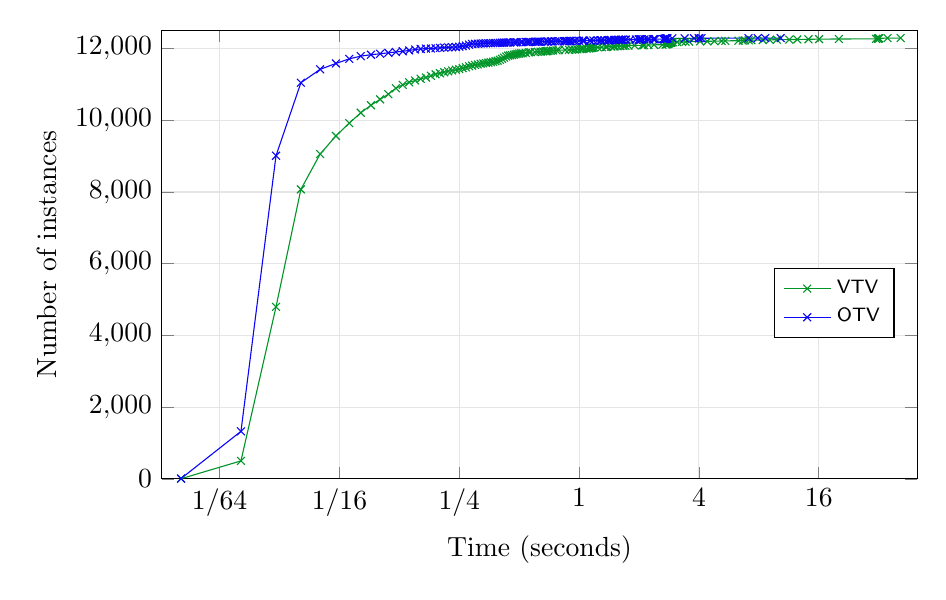
\begin{tikzpicture}[scale = 1.0]
    \begin{axis}
      [
        mark options={scale=1.0},
        grid=both, 
        grid style={black!10}, 
        xmode=log, 
        % ymode=log, 
        legend style={at={(0.97,0.47)}}, 
        legend cell align={left},
        x post scale=1.4, 
        y post scale=1.0, 
        xlabel=Time (seconds), 
        ylabel=Number of instances, 
        xtick={1000/64, 1000/16, 1000/4, 1000, 4000, 16000, 64000, 256000},
        xticklabels={1/64, 1/16, 1/4, 1, 4, 16, 64, 256},
        xmin=8,
        xmax=50000,
        ymin=0,
        ymax=12500, 
        scaled x ticks=false,
        scaled y ticks=false,
      ]

      \addplot[color=VTV, mark=x] coordinates { 
        (10, 5) (20, 502) (30, 4797) (40, 8072) (50, 9059) (60, 9562)
        (70, 9920) (80, 10208) (90, 10419) (100, 10582) (110, 10725) (120, 10892)
        (130, 10986) (140, 11057) (150, 11108) (160, 11156) (170, 11192) (180, 11239)
        (190, 11280) (200, 11310) (210, 11339) (220, 11365) (230, 11386) (240, 11409)
        (250, 11425) (260, 11451) (270, 11476) (280, 11504) (290, 11522) (300, 11543)
        (310, 11556) (320, 11574) (330, 11586) (340, 11594) (350, 11606) (360, 11620)
        (370, 11630) (380, 11646) (390, 11660) (400, 11685) (410, 11713) (420, 11744)
        (430, 11775) (440, 11801) (450, 11810) (460, 11816) (470, 11827) (480, 11840)
        (490, 11853) (500, 11860) (510, 11864) (520, 11869) (540, 11877) (560, 11891)
        (570, 11897) (600, 11901) (620, 11908) (640, 11912) (660, 11918) (680, 11923)
        (690, 11927) (700, 11931) (720, 11939) (740, 11943) (770, 11949) (790, 11953)
        (850, 11958) (890, 11962) (920, 11967) (950, 11971) (980, 11977) (1010, 11981)
        (1030, 11985) (1050, 11990) (1090, 11994) (1120, 12002) (1130, 12008) (1150, 12013)
        (1160, 12021) (1170, 12025) (1190, 12029) (1240, 12033) (1300, 12037) (1360, 12041)
        (1380, 12046) (1450, 12051) (1490, 12055) (1510, 12059) (1560, 12063) (1610, 12068)
        (1670, 12072) (1710, 12076) (1770, 12081) (1900, 12085) (2080, 12089) (2120, 12093)
        (2230, 12097) (2380, 12102) (2620, 12106) (2720, 12110) (2740, 12114) (2760, 12120)
        (2780, 12124) (2800, 12130) (2810, 12137) (2840, 12146) (2870, 12155) (2890, 12161)
        (2900, 12167) (2920, 12171) (2960, 12175) (3110, 12179) (3290, 12184) (3430, 12188)
        (3570, 12193) (4050, 12197) (4400, 12201) (4780, 12205) (5200, 12209) (5420, 12213)
        (6320, 12217) (6640, 12221) (6790, 12225) (7110, 12229) (7340, 12233) (8370, 12237)
        (9080, 12241) (9860, 12245) (11370, 12249) (12480, 12253) (14200, 12257) (16070, 12261)
        (20190, 12265) (31050, 12269) (31670, 12273) (31840, 12277) (31980, 12281) (32130, 12285)
        (35440, 12289) (41260, 12291)
      };

      \addplot[color=OTV, mark=x] coordinates { 
        (10, 10) (20, 1326) (30, 9011) (40, 11045) (50, 11419) (60, 11583)
        (70, 11711) (80, 11787) (90, 11827) (100, 11853) (110, 11879) (120, 11903)
        (130, 11922) (140, 11946) (150, 11973) (160, 11987) (170, 11998) (180, 12000)
        (190, 12010) (200, 12017) (210, 12025) (220, 12031) (230, 12036) (240, 12042)
        (250, 12049) (260, 12065) (270, 12082) (280, 12107) (290, 12127) (300, 12131)
        (310, 12134) (320, 12138) (330, 12142) (340, 12145) (350, 12147) (360, 12149)
        (370, 12150) (380, 12154) (390, 12157) (400, 12160) (410, 12161) (420, 12164)
        (430, 12165) (440, 12167) (450, 12168) (470, 12171) (480, 12173) (490, 12174)
        (510, 12177) (520, 12179) (540, 12180) (550, 12181) (560, 12182) (570, 12186)
        (600, 12187) (610, 12188) (620, 12189) (630, 12190) (640, 12192) (670, 12193)
        (690, 12194) (700, 12195) (720, 12197) (730, 12199) (760, 12200) (780, 12201)
        (800, 12202) (840, 12203) (850, 12205) (860, 12206) (870, 12207) (890, 12208)
        (900, 12209) (910, 12211) (940, 12213) (960, 12214) (1000, 12215) (1040, 12217)
        (1050, 12218) (1060, 12219) (1130, 12220) (1140, 12221) (1180, 12223) (1240, 12224)
        (1280, 12225) (1290, 12226) (1300, 12227) (1340, 12228) (1400, 12230) (1410, 12232)
        (1420, 12233) (1440, 12234) (1450, 12236) (1500, 12237) (1520, 12238) (1530, 12239)
        (1570, 12240) (1590, 12241) (1620, 12242) (1630, 12243) (1650, 12244) (1660, 12245)
        (1710, 12246) (1720, 12247) (1810, 12249) (1930, 12250) (2000, 12251) (2010, 12252)
        (2020, 12253) (2050, 12254) (2060, 12255) (2130, 12256) (2200, 12257) (2240, 12258)
        (2360, 12259) (2380, 12260) (2410, 12261) (2650, 12262) (2660, 12263) (2680, 12264)
        (2690, 12268) (2700, 12269) (2710, 12270) (2720, 12274) (2730, 12277) (2740, 12278)
        (2760, 12279) (2770, 12280) (2780, 12281) (2940, 12282) (3390, 12283) (3780, 12284)
        (3990, 12285) (4020, 12286) (4120, 12287) (7100, 12288) (7900, 12289) (8610, 12290)
        (10300, 12291)
      };
    
      \legend{
        \scriptsize \textsf{VTV}, 
        \scriptsize \textsf{OTV}
      }
    
    \end{axis}
  \end{tikzpicture}

  \caption{
    Verification times of VTV and OTV. The datapoints show the number of TESC proofs 
    that each verifier could check within the given time limit. The plots look more 
    ``jumpy'' toward the lower end due to the limited  time measurement resolution (10 ms) 
    of the unix \texttt{time} command.
  }
  \label{fig:time}
\end{figure}

VTV is slower than OTV as expected, but the difference is unlikely
to be noticed in actual use since the total times are dominated by a few 
outliers and the absolute times for most proofs are very short: the median 
time for VTV is 40 ms, a mere 10 ms behind the OTV's 30 ms. Also,
VTV verified >97.4\% of proofs under 1 second, and >99.3\% under 5 seconds. 
But OTV's mean time (54.54 ms) is still much shorter than that of VTV (218.93 ms),
so users may prefer OTV for verifying one of the hard outliers or processing
a large batch of proofs at once.

The main drawback of VTV is its high memory consumption. Fig. \ref{fig:mem} shows
the peak memory usages of the two verifiers. For a large majority of proofs, 
memory usage for both verifiers are stable and stays within the 14-20 MB range,
but VTV's memory usage spikes both earlier and higher than OTV. Due the limit of 
the system used, memory usage could only be measured up to 16 GB, but the actual peak for VTV 
would be higher if we included the 5 failed verifications. A separate test running 
VTV on an EC2 instance with 64 GB ram (\texttt{r5a.2xlarge}) still failed for 3 of 
the 5 problematic proofs, so the memory requirement for verifying all 12296 proofs 
with VTV is at least >64 GB. In contrast, OTV could verify all 
12296 proofs with less than 3.2 GB of memory.

\begin{figure}[tb]
  \centering
  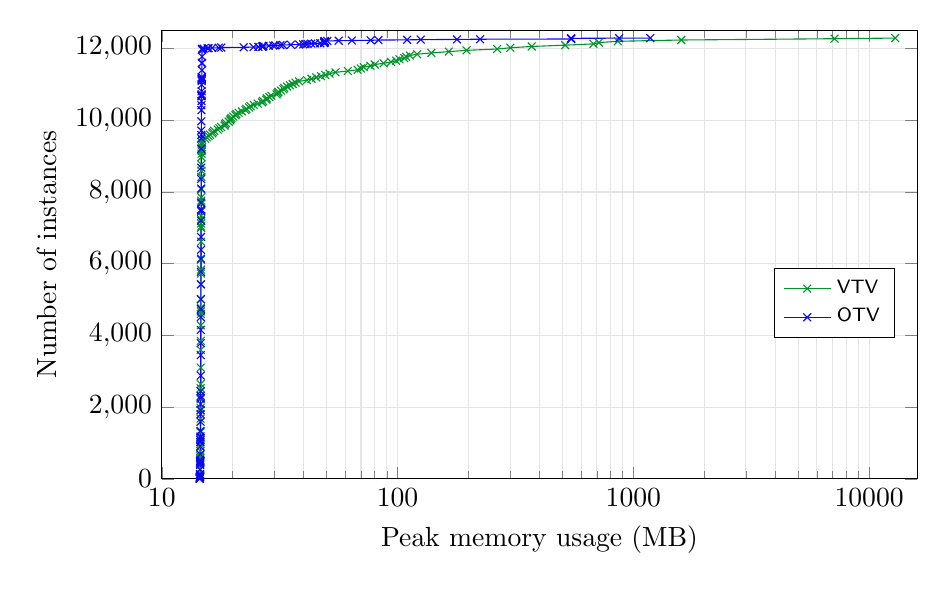
\begin{tikzpicture}[scale = 1.0]
    \begin{axis}
      [
        mark options={scale=1.0},
        grid=both, 
        grid style={black!10}, 
        xmode=log, 
        % ymode=log, 
        legend style={at={(0.97,0.47)}}, 
        legend cell align={left},
        x post scale=1.4, 
        y post scale=1.0, 
        xlabel=Peak memory usage (MB), 
        ylabel=Number of instances, 
        xtick={10000, 100000, 1000000, 10000000},
        xticklabels={10, 100, 1000, 10000},
        xmin=10000,
        xmax=16000000,
        ymin=0,
        ymax=12500, 
        scaled x ticks=false,
        scaled y ticks=false,
      ]

      \addplot[color=VTV, mark=x] coordinates { 
        (14472, 4) (14512, 55) (14536, 104) (14544, 277) (14548, 501) (14556, 573)
        (14564, 625) (14568, 673) (14572, 771) (14576, 894) (14584, 972) (14588, 1022)
        (14592, 1082) (14596, 1300) (14600, 1679) (14604, 1910) (14608, 1976) (14612, 2218)
        (14616, 2448) (14620, 2528) (14624, 2645) (14628, 3104) (14632, 3595) (14636, 3849)
        (14640, 4282) (14644, 4598) (14648, 4671) (14652, 4771) (14656, 5013) (14660, 5430)
        (14664, 5724) (14668, 5837) (14672, 6105) (14676, 6612) (14680, 6999) (14684, 7036)
        (14688, 7120) (14692, 7240) (14696, 7331) (14700, 7497) (14704, 7679) (14708, 7757)
        (14716, 7850) (14720, 8067) (14724, 8421) (14728, 8590) (14732, 8766) (14736, 8974)
        (14752, 9066) (14756, 9136) (14780, 9177) (14800, 9244) (14804, 9320) (14812, 9379)
        (14816, 9451) (15260, 9487) (15516, 9524) (15792, 9560) (16032, 9597) (16376, 9633)
        (16500, 9669) (16672, 9705) (17264, 9741) (17552, 9777) (17852, 9813) (18484, 9849)
        (18580, 9886) (18692, 9922) (19232, 9958) (19532, 9994) (19596, 10030) (19748, 10066)
        (20092, 10102) (20544, 10138) (20724, 10174) (21184, 10210) (21864, 10246) (22644, 10282)
        (22864, 10319) (23464, 10355) (23792, 10392) (24548, 10428) (25520, 10464) (26620, 10500)
        (26872, 10536) (27752, 10573) (27904, 10610) (28576, 10646) (29144, 10682) (30688, 10718)
        (30944, 10754) (31228, 10790) (32044, 10827) (32824, 10863) (33072, 10903) (33988, 10939)
        (34940, 10975) (35920, 11011) (36920, 11047) (38176, 11083) (41308, 11119) (43172, 11156)
        (45212, 11192) (47408, 11228) (49396, 11264) (51452, 11300) (54560, 11336) (61516, 11372)
        (67676, 11408) (69864, 11444) (71908, 11481) (76712, 11517) (80040, 11553) (87340, 11589)
        (93824, 11625) (98492, 11661) (101808, 11697) (106604, 11733) (108720, 11769) (112800, 11805)
        (121040, 11841) (139104, 11877) (164980, 11913) (196100, 11949) (264488, 11985) (300696, 12021)
        (370688, 12057) (513672, 12093) (677000, 12129) (714032, 12165) (859376, 12201) (1596720, 12237)
        (7129160, 12273) (12897180, 12291)
      };

      \addplot[color=OTV, mark=x] coordinates { 
        (14472, 6) (14496, 13) (14504, 28) (14508, 37) (14512, 48) (14524, 57)
        (14528, 68) (14532, 74) (14536, 107) (14540, 135) (14544, 253) (14548, 389)
        (14552, 424) (14556, 452) (14560, 474) (14564, 498) (14568, 535) (14572, 687)
        (14576, 912) (14580, 1030) (14584, 1076) (14588, 1145) (14592, 1183) (14596, 1336)
        (14600, 1594) (14604, 1804) (14608, 1914) (14612, 2089) (14616, 2254) (14620, 2314)
        (14624, 2441) (14628, 2881) (14632, 3452) (14636, 3785) (14640, 4155) (14644, 4511)
        (14648, 4733) (14652, 5010) (14656, 5422) (14660, 5776) (14664, 6142) (14668, 6386)
        (14672, 6746) (14676, 7199) (14680, 7461) (14684, 7512) (14688, 7706) (14692, 8095)
        (14696, 8361) (14700, 8679) (14704, 9205) (14708, 9491) (14712, 9591) (14716, 9712)
        (14720, 9969) (14724, 10281) (14728, 10418) (14732, 10533) (14736, 10666) (14740, 10681)
        (14744, 10696) (14748, 10722) (14752, 10807) (14756, 10991) (14760, 11093) (14764, 11124)
        (14768, 11146) (14776, 11154) (14780, 11176) (14784, 11195) (14792, 11206) (14800, 11396)
        (14804, 11590) (14808, 11600) (14812, 11773) (14816, 11966) (14820, 11979) (14832, 11985)
        (14836, 11991) (15072, 11997) (15620, 12003) (15796, 12009) (16364, 12015) (17436, 12021)
        (17880, 12027) (22252, 12033) (24480, 12039) (25684, 12045) (26656, 12051) (26752, 12057)
        (26880, 12063) (26956, 12069) (28436, 12075) (29684, 12081) (30296, 12087) (31860, 12093)
        (32656, 12099) (35272, 12105) (38244, 12111) (39820, 12117) (40676, 12123) (41460, 12129)
        (43032, 12135) (44632, 12141) (46996, 12147) (48872, 12154) (48900, 12161) (48924, 12168)
        (48956, 12175) (48964, 12181) (48996, 12187) (49032, 12193) (49088, 12199) (49116, 12205)
        (50372, 12211) (56284, 12217) (63976, 12223) (76892, 12229) (82960, 12235) (109728, 12241)
        (125312, 12247) (178576, 12253) (224040, 12259) (544396, 12265) (544488, 12271) (544532, 12277)
        (544688, 12283) (870444, 12289) (1179916, 12291)
      };
    
      \legend{
        \scriptsize \textsf{VTV}, 
        \scriptsize \textsf{OTV}
      }
    
    \end{axis}
  \end{tikzpicture}

  \caption{
    Peak memory usages of VTV and OTV. The datapoints show the number of TESC proofs 
    that each verifier could check within the given peak memory usage. 
  }
  \label{fig:mem}
\end{figure}

\section{Conclusion}  \label{sec:conclusion}

VTV can serve as a fallback option whenever extra rigour is required in verification, 
thereby increasing our confidence in the correctness of TESC proofs. 
It also helps the design of other TESC verifiers by providing a reference 
implementation that is guaranteed to be correct. It should be particularly helpful 
for implementing other verified TESC verifiers in, say, Lean or Coq, since many 
of the issues we've discussed (termination checking, data structures, etc.) 
are common to these languages. 

There are two main ways in which VTV could be further improved. Curbing its 
memory usage would be the most important prerequisite for making it the 
default verifier in T3P. This may require porting VTV to a verified programming
language with finer low-level control over memory usage. 

VTV could also benefit from a more reliable TPTP parser. A formally verified 
parser would be ideal, but the complexity of TPTP's syntax makes it difficult  
to even \textit{specify} the correctness of a parser, let alone prove it. 
A more realistic approach would be imitating the technique used by verified 
LRAT checkers \cite{heule2017efficient}, making VTV print the parsed problem 
and textually comparing its with the original problem.

\bibliographystyle{plain}

\bibliography{references}

\end{document}

















